\chapter{Evaluation}
By importing ModelDBSyncer and appending "Sync" to the method names, the user
can use ModelDB Spark Client to record and send their operations and models
on ModelDB Server, which stores the data in its database and model filesystem.
Naturally, this takes extra running time and storage space than if the user did
not ModelDB S+C at all. Additionally, the API methods exposed by ModelDB Server
take some time to run too. The goal of this chapter is to measure whether the time
and space requirements of ModelDB S+C are reasonable.


\section{Overview}
Experiments were conducted to answer the following questions:

\begin{enumerate}
\item Is the time overhead of storing operations and models on ModelDB Server reasonably small (compared to
the overall running time of the Spark.ML program)?
\item Is the space taken up by ModelDB S+C's database and model files reasonably small (compared
to the size of the dataset)?
\item Are ModelDB S+C's tree model and linear model representations reasonably small (compared 
to the size of corresponding PMML files)?
\item Is the time take to execute the ModelDB Server API methods reasonably small (compared
to the training time of the model)?
\item Can ModelDB S+C record most of the machine learning operations in real Spark.ML programs?
\end{enumerate}

The chapter also discusses performance improvements that can further improve ModelDB S+C with
regard to the above questions.

\section{Datasets}
ModelDB S+C was evaluated on real datasets, which are described below:

The \textbf{IMDB} dataset \cite{imdb} includes features like genre, number of
reviews, language, and more for over 5000 movies in the IMDB Movie Database. The dataset
also includes the IMDB score (i.e. a 1 to 10 rating of how good the movie is considered)
for each movie. A machine learning model could solve a regression problem on this
dataset in which it predicts the IMDB score for a given movie. Such a model could, for instance,
be used to identify the best movies and recommend them to users. This dataset
was used when measuring the time/space overhead of ModelDB S+C and was also used
when measuring the execution time for ModelDB Server API methods.

The \textbf{Animal Shelter} dataset \cite{animal} includes features like
animal type (cat or dog), breed, color, age, and more for over 25,000 animals. The
dataset also includes the animal's outcome (e.g. adopted, returned to owner, transferred)
for each animal. A machine learning model could solve a multi-class classification problem on this dataset
in which it predicts the most likely outcome for a given animal. Such a model could, for
instance, be used to identify the most likely outcome for an animal newly admitted into the
an animal shelter. This dataset was used when measuring the time/space overhead
of ModelDB S+C.

The \textbf{Housing Prices} dataset \cite{housing} includes features like square
footage, number of bathrooms, neighborhood type, and more for about 1,500 houses.
The dataset also includes the sale price of each house. A machine learning model
could solve a regression problem on this dataset in which it predicts the sale
price of a given home. Such a model could, for instance, be used by realtors who
are trying to find the best price for a home when putting it up on the market. This
dataset was used when measuring the time/space overhead of ModelDB S+C.

The \textbf{Iris} dataset \cite{iris} is a famous dataset that includes features
like petal length, sepal width, and more for 150 Iris plans. The dataset also
includes the species of the Iris plant. A machine learning model could solve a 
multi-class classification problem on this dataset in which it predicts the species
of a given Iris plant. Such a model may be useful for botanists looking to classify
their plants. This dataset was used when measuring the size of ModelDB S+C models
to PMML models (the PMML website includes model files for the Iris dataset).

The \textbf{Titanic} dataset \cite{titanic} is a famous dataset includes features like 
passenger sex, passenger class, and more for over 1300 passengers of the Titanic. 
The dataset also includes whether each passenger survived or died. A machine learning
model could solve a binary classification problem on this dataset in which it predicts whether
a given passenger survived. Such a model may be useful for historians. This dataset
was used when evaluating ModelDB S+C on an existing machine learning workflow.

The \textbf{SMS Spam} dataset \cite{spam} includes over 5500 text messages and
a label indicating whether the message is spam or not. A machine learning model
could solve a binary classification problem on this dataset in which it predicts
whether a given text message is spam. Such a model could be used as a text messaging
app's spam filter. This dataset was used when evaluating ModelDB S+C on an existing
machine learning workflow.

The \textbf{Flight Delays} dataset \cite{airline} includes features like carrier, departure
time, and more for over 14 million airplane departures. It also includes a field indicating whether
the plane was delayed. A machine learning model could solve a binary classification problem on this dataset in which
it predicts whether a given airplane is delayed. Such a model could be used by airports and airlines
to anticipate delays for particular airplanes. This dataset was used when evaluating ModelDB S+C
on an existing machine learning workflow.

\section{Methodology}
\subsection{Machine}
These experiments were run on a DigitalOcean machine with a 160 GB SSD disk, an 8 core processor,
and 16GB of memory.

\subsection{Time and Space Overhead}
The first experiment focused on evaluating the time and space overhead of ModelDB S+C.
The IMDB, Housing Prices, and Animal Shelter datasets were used for this experiment. 

First, for each of the datasets listed above, three programs (called workflows) were
created. The \textbf{simple} workflow simply trains and evaluates one machine learning model. 
The \textbf{full} workflow creates a preprocessing pipeline for the data, trains 
some models with grid search cross validation (thus trying many hyperparameters), 
and evaluates the best model. The \textbf{exploratory} worklow executes many full workflows, 
trying different model types (e.g. random forest, linear regression) and different feature sets.

Second, a program was written to artificially increase the size of the dataset by duplicating rows.
Dataset sizes were varied from the dataset's original number of rows to one million rows.

Third, ModelDB Spark Client was instrumented so that it recorded the time spent running code related
to ModelDB S+C.

Fourth, each (dataset, dataset size, workflow) triple's program was executed with ModelDB S+C enabled. The time that ModelDB S+C spent
recording and storing each operation and model was recorded. The database size, number of rows in each table, and size of the model
files was also recorded. Finally, the overall running time of the program and the size of the (artificially enlarged) dataset
were also noted. Due to Spark's large memory requirements, it was not possible to run the exploratory workflow for the 
housing dataset when the number of rows was large because Spark.ML consumed too much memory. This is because Spark is designed
to be run on machines with large amounts of RAM, and the machine used for these experiments had only 16 GB of RAM.

\subsection{Computation Time of API Methods}
The second experiment focused on evaluating the running time of ModelDB Server's API methods. The
IMDB dataset was used here.

First, the IMDB exploratory workflow was run to populate ModelDB Server's database.

Second, the database was duplicated $N$ times (i.e. $N$ additional rows were created for
every row in every table of the database), where $N$ was varied from 0 to 400. This was
done to simulate many exploratory workflows being run on ModelDB S+C.

Third, various API methods were executed on the (artificially enlarged) database and the
running time for each method was recorded.

\subsection{Compare ModelDB S+C Models to PMML}
The PMML website \cite{pmmlwebsite} includes sample files for a 200 tree random forest model
and logistic regression model run that were trained on the Iris dataset. So, this
experiment trained a random forest model and one vs. rest logistic regression model
in Spark.ML (with ModelDB S+C enabled). The sizes of the model files and database
were recorded.

\subsection{Evaluating Existing Workflows}
Three machine learning workflows were collected from the Internet. The first \cite{flightworkflow}, from
a Hortonworks article, uses the Flight Delays dataset to build a regression model to predict
delays. The second \cite{titanicworkflow} and third \cite{spamworkflow} are from ZeppelinHub, a website that allows users to share their
machine learning workflows as Zeppelin notebooks. The second workflow trains two models
to predict passenger survival status for the Titanic dataset and the third builds a spam classifier
using the SMS Spam dataset. These workflows were cleaned up, ported to Spark v2.0.0, and 
augmented with ModelDB Spark Client (i.e. import ModelDbSyncer and add *Sync to the methods).

\section{Time Overhead Results}
To measure the time overhead, the time spent running ModelDB S+C code is divided 
by the total running time of the program and the result is taken as a percentage.
Plotting this time overhead percentage, for each (dataset, workflow) pair,
as a function of the number of rows in the dataset yields Figure \ref{fig:time_overhead}.
For this experiment, ModelDB S+C did NOT count the number of rows in each DataFrame.

\begin{figure}
  \centering
  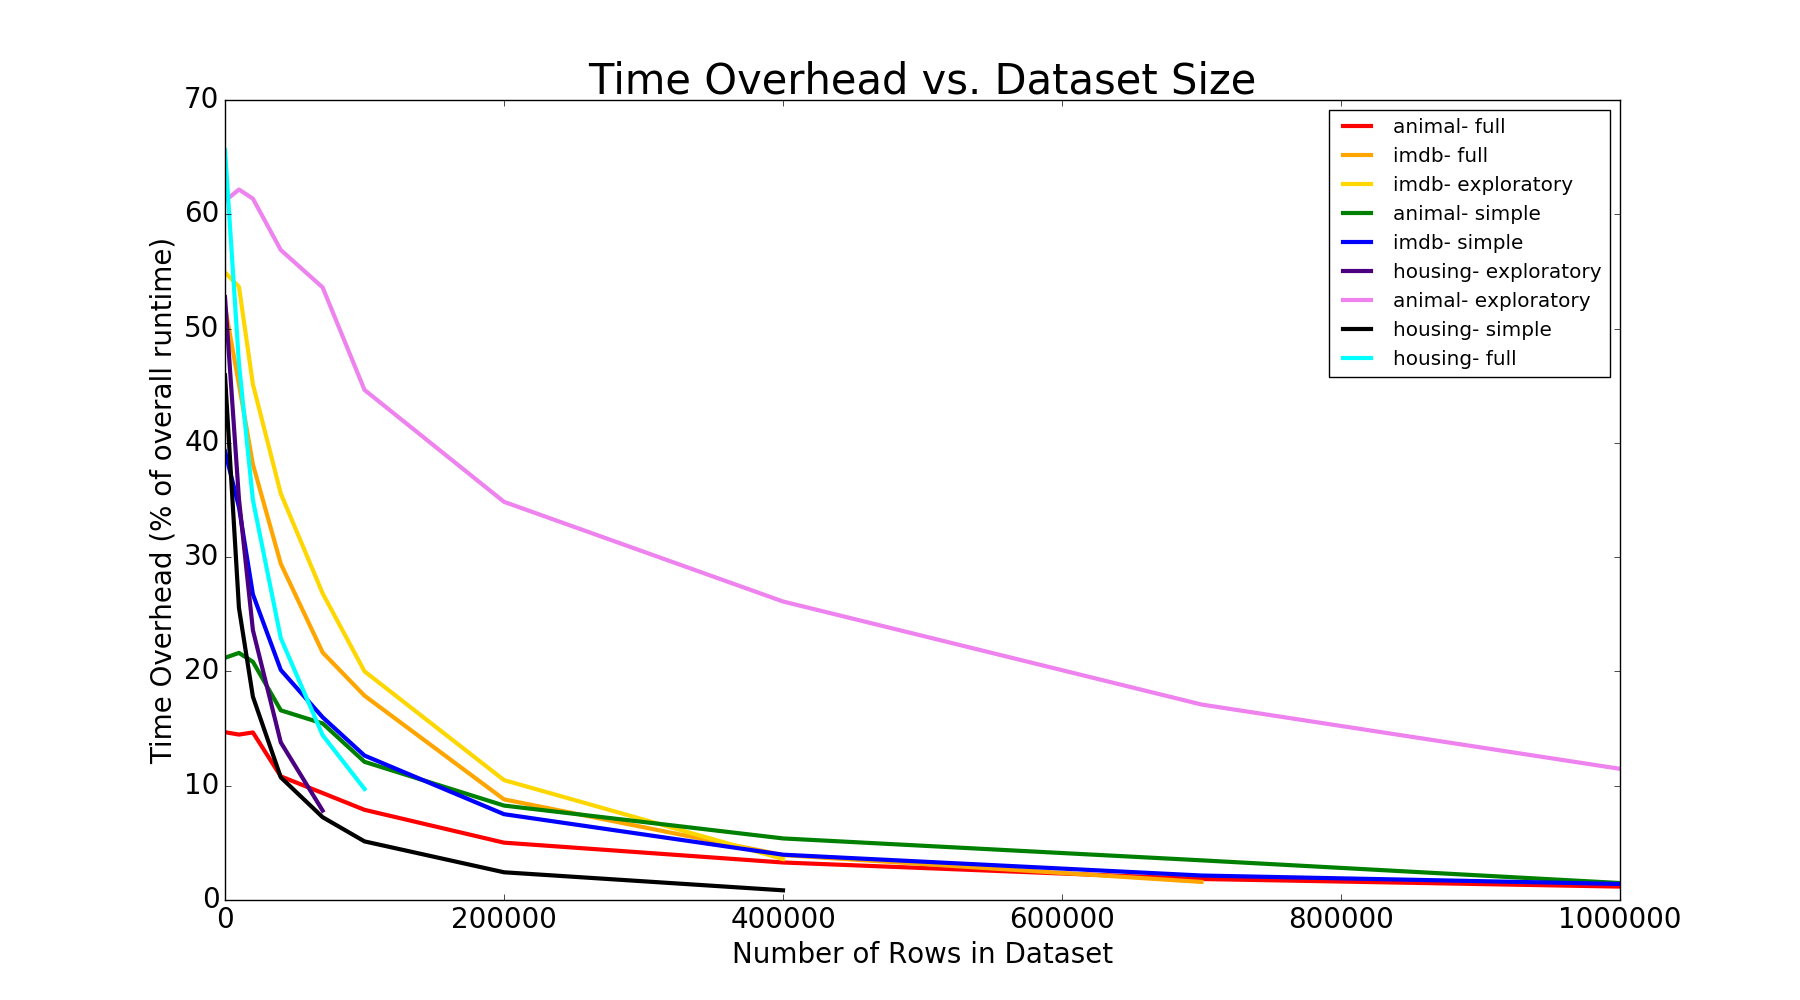
\includegraphics[width=6.0in]{time_overhead}
  \caption{
    Time overhead of ModelDB S+C.
  }
  \label{fig:time_overhead}
\end{figure}

Figure \ref{fig:time_overhead} shows that, as the dataset size grows, the time overhead
percentage for ModelDB S+C goes down. For a one million row dataset,
most of the workflows spend less than 5\% of their time running ModelDB S+C code.

For the results here, ModelDB S+C is configured not to count the number of rows in the DataFrames.
Counting the number of rows in a Spark DataFrame requires a sequential scan of the DataFrame. Doing this
would cause the absolute time spent running ModelDB S+C code to grow linearly with the dataset size. So, ModelDB Spark
Client disables row-counting by default.

In Figure \ref{fig:time_overhead}, the dataset size is measured in number of rows, rather than in
the actual size of the data file. This is done because the file format of the data has a big impact on
the size of the data file. Nevertheless, for reference, the largest dataset size (1 million rows) was under 300 MB
in size. All data was in CSV format.

Thus, Figure \ref{fig:time_overhead} shows that the time overhead of ModelDB S+C becomes insignificant 
as the dataset grows beyond 300 MB. 

The slowest step in recording and storing a model or operation, as determined yby 
instrumenting various lines of code, is writing to the SQLite database. This is not a surprise
because the SQLite file lives on disk and because SQLite is not a very performant database.
Replacing SQLite with a more performant database may not only reduce the time overhead, it may
also reduce the storage requirements as well if data is appropriately compressed.

Focusing on the individual operations, the operation that consumed the most time, by far, was
GridSearchCrossValidationEvent. The average time overhead percentages for the most time
consuming operations are shown in Figure \ref{fig:event_time_overhead}.

\begin{figure}
  \centering
  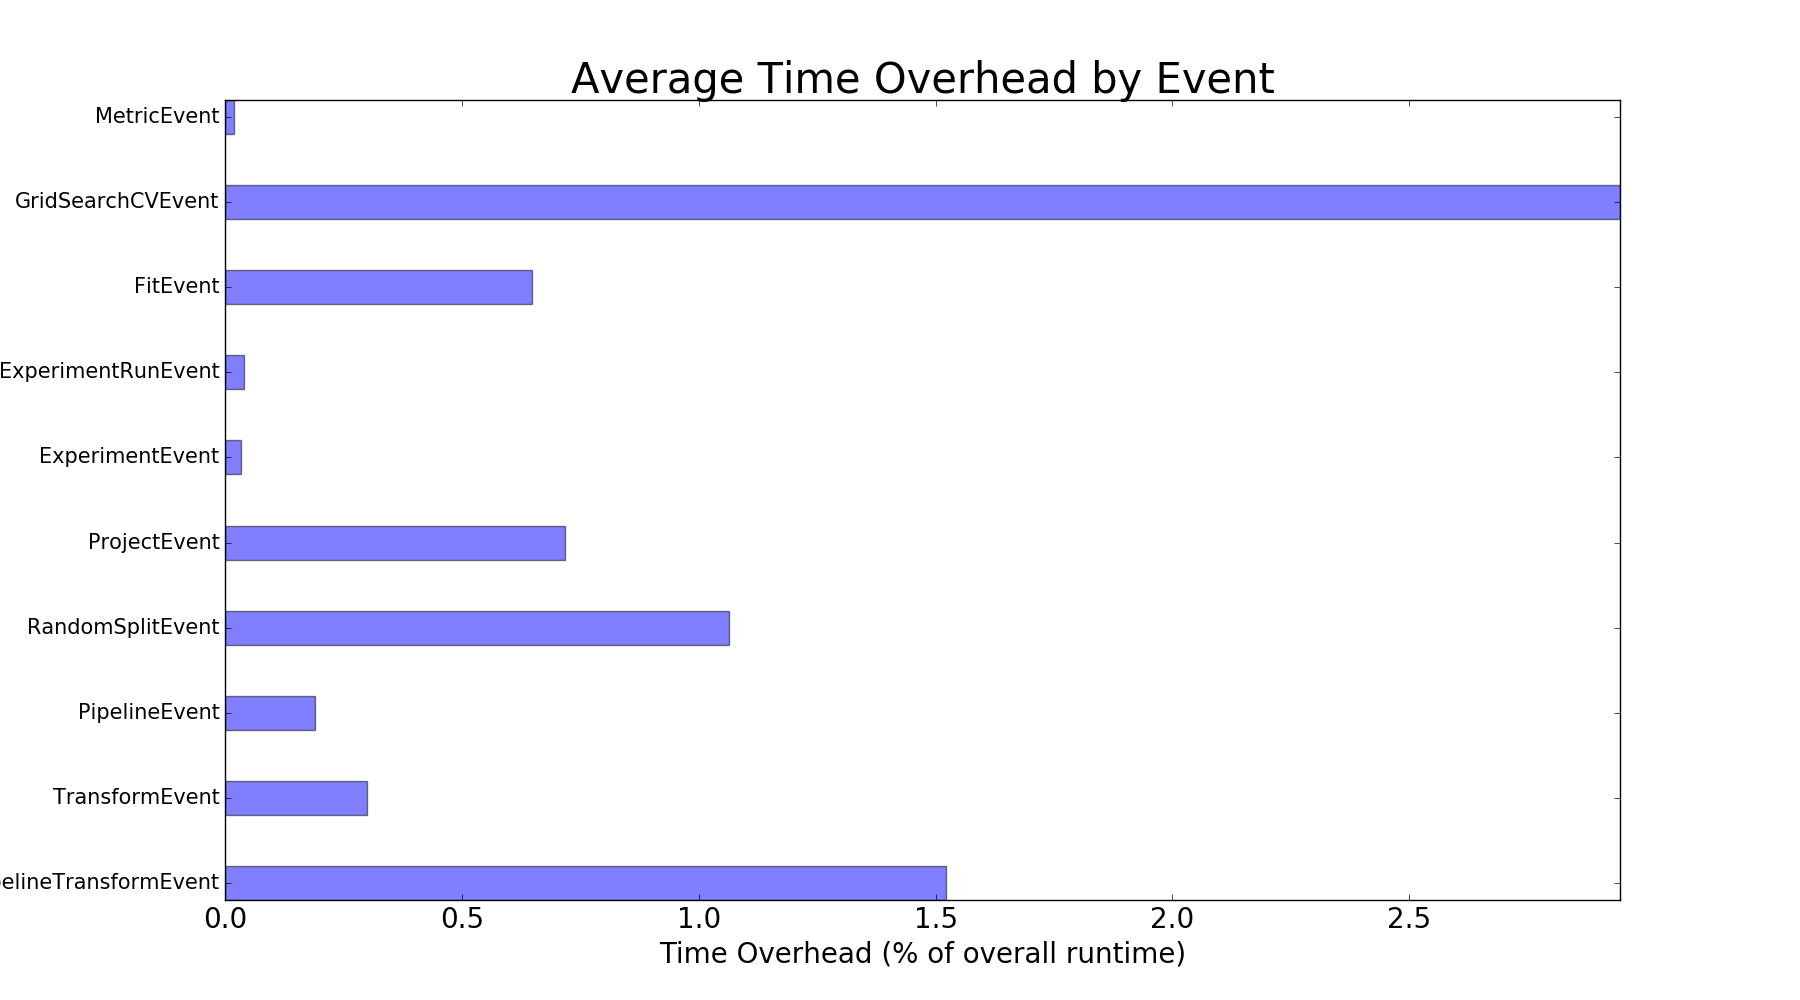
\includegraphics[width=6.0in]{event_time_overhead}
  \caption{
    Average time overhead percentage by event.
  }
  \label{fig:event_time_overhead}
\end{figure}

Figure \ref{fig:event_time_overhead} shows that roughly 3\% of the time in the overall
program is spent storing GridSearchCrossValidationEvents. This occurs because a GridSearchCrossValidationEvent
has many other smaller events contained inside it, such as TransformEvents, FitEvents, MetricEvents, and 
CrossValidationEvents. Consequently, ModelDB Server has to write many rows to many database tables when a
GridSearchCrossValidationEvent occurs. If the user is not interested in storing all the intermediate FitEvents,
TransformEvents, etc. for a GridSearchCrossValidation, then much of this overhead is a waste. Therefore, ModelDB S+C
allows the user to configure whether they would like to actually store all the data associated with a GridSearchCrossValidationEvent,
or whether they would like to simply store the FitEvent associated with the produced model. This makes it possible to cut out
much of the overhead caused by GridSearchCrossValidationEvents.

Thus, to summarize, ModelDB S+C's time overhead is small when the dataset is large (i.e. 300 MB or more). A
large fraction of the time is spent storing GridSearchCrossValidationEvents, and since the user may not
care about storing all the intermediate TransformEvents, MetricEvents, etc., the user is allowed to indicate 
whether they would like to store the full event or or just the FitEvent for the produced model.

\section{Storage Overhead Results}
For a fixed (dataset, workflow) pair, the size of ModelDB S+C's database and the size of the
model files do not change even as the number of rows in the dataset changes. This makes sense
because, except for counting the number of rows, ModelDB S+C does not access any data from the
DataFrame's rows. The size of ModelDB S+C's SQLite database is shown for each of the (dataset, workflow)
pairs in Figure \ref{fig:dbsize}.

\begin{figure}
  \centering
  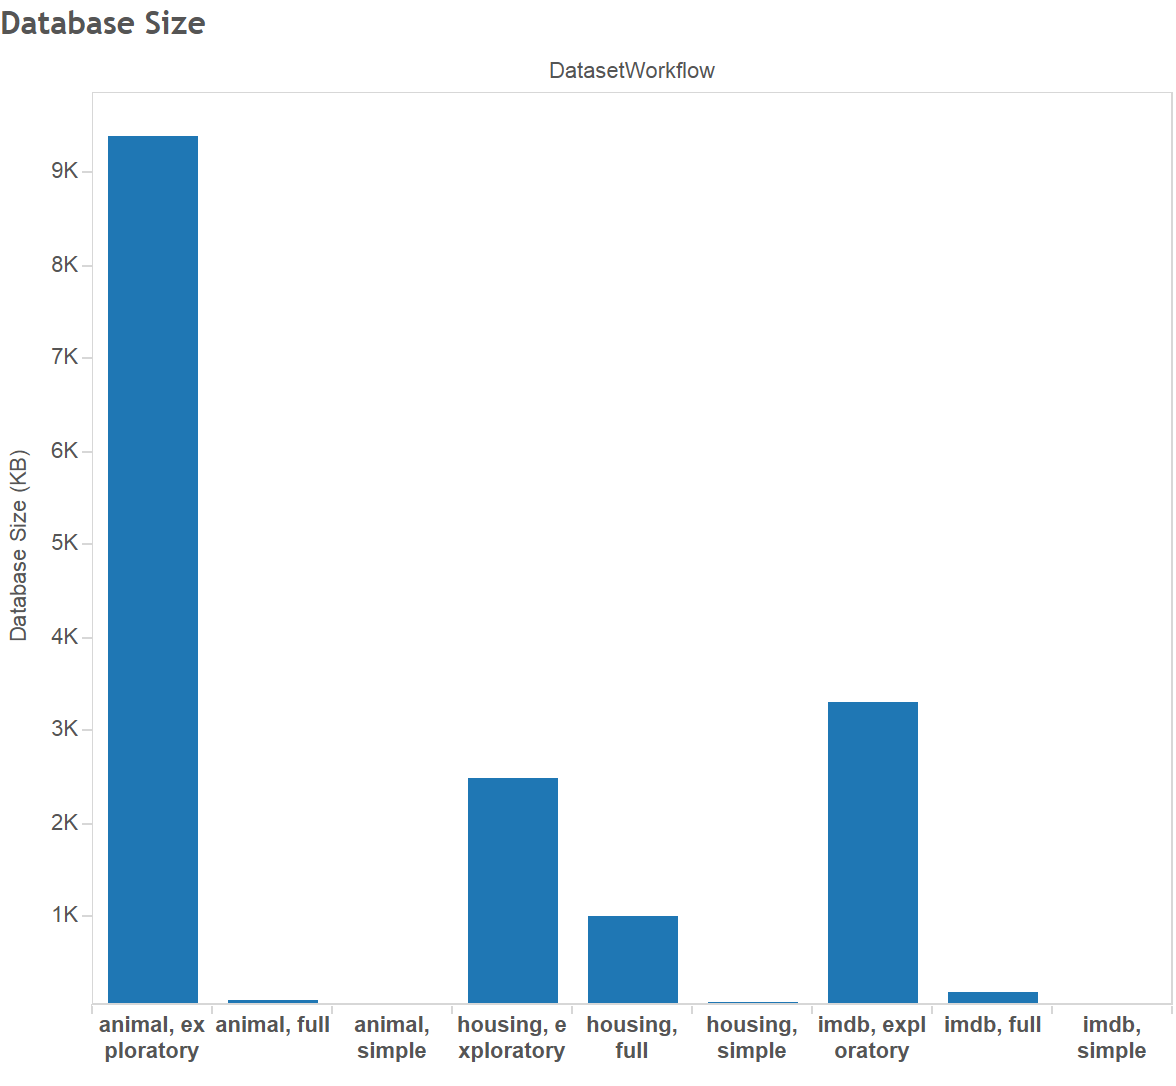
\includegraphics[height=4.0in]{dbsize}
  \caption{
    Database size (in KB) for each (dataset, workflow) pair.
  }
  \label{fig:dbsize}
\end{figure}

For all the (dataset, workflow) pairs, the database size remains under 10MB, and is
just a few MB for most of the (dataset, workflow) pairs. Since machine learning datasets
tend to be large (e.g. several hundred GB), 10MB is quite small. That being said, inspecting
the number of rows in each table for the Animal Shelter exploratory workflow 
can provide some insight into reducing the database size even further. This is shown in Figure
\ref{fig:animal_exploratory_table_sizes}.

\begin{figure}
  \centering
  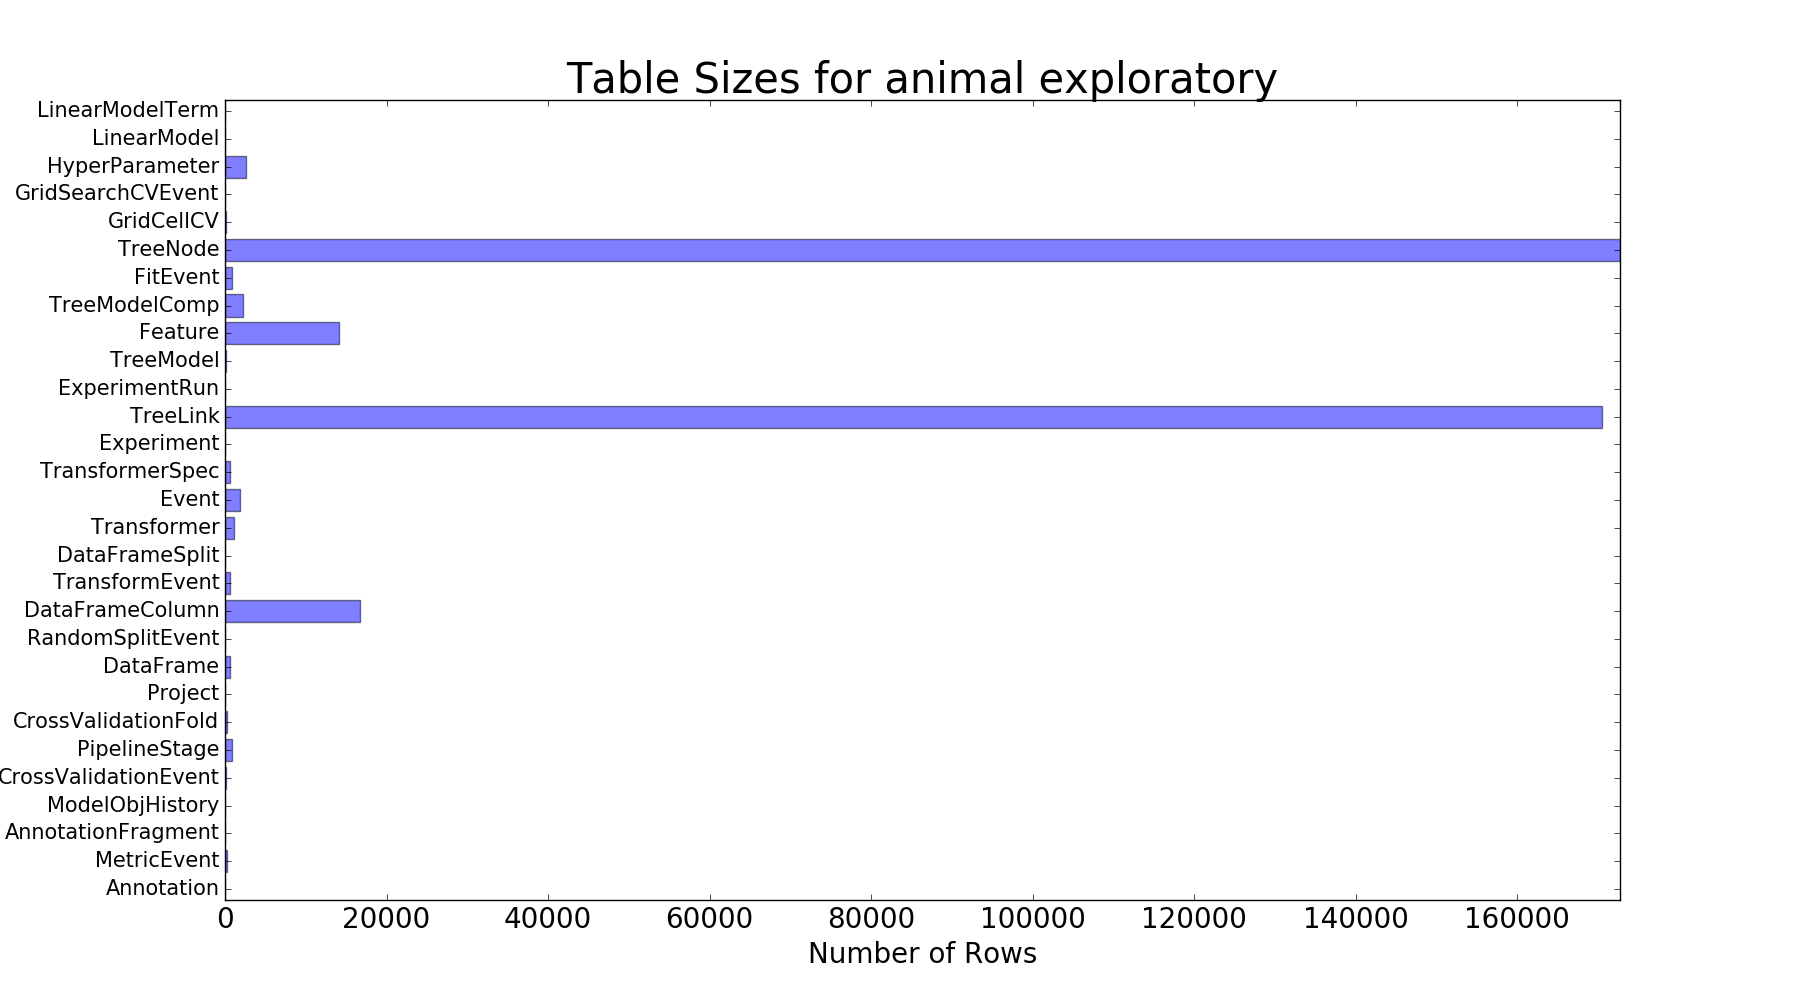
\includegraphics[width=6.0in]{animal_exploratory_table_sizes}
  \caption{
    Size of tables (in number of rows) for exploratory workflow for Animal
    Shelter dataset.
  }
  \label{fig:animal_exploratory_table_sizes}
\end{figure}

Overwhelmingly, the TreeModel and TreeLink tables have the most rows. A little
thought, however, shows that this is not surprising. The Animal Shelter exploratory workflow
trains a number of random forest models. Consider
a random forest with 20 decision trees where each tree has depth 7. Further assume
that each decision tree is a binary tree. This means that each tree has on the
order of $2^{7} = 128$ nodes (and roughly the same number of links). Thus, the
random forest has $20 \times 128 = 2650$ nodes (and roughly the same number of links).
If 3-fold grid search cross validation is conducted with 8 hyperparameter configurations (a $4 \times 2$ 
search grid), and a total of 3 such grid search cross validations are performend, 
this becomes $2650 \times 8 \times 3 \times 3 = 190,800$ nodes (and roughly the same number of links).
Therefore, it is no surprise that the TreeNode and TreeLink tables are so large.

ModelDB S+C provides two mechanisms to reduce database size. First, as described before, it
allows the user to forgo storing ALL the data associated with a GridSearchCrossValidationEvent and instead
store only the most important parts.
Second, it allows the user to forgo storing storing entries in the TreeLink and TreeNode table (the
node and link data are already stored in the serialized model file) except for specified models. This can reduce the database size
greatly, and allow the user to only store TreeNode and TreeLink rows when it is necessary. In the 
exploratory workflow for the Animal Shelter workflow, only one (i.e. the best)  model's TreeLink and TreeNode data is really needed,
but the workflow stores data for dozens of random forest models. When the above two mechanisms are applied,
the size of the database falls from about 9 MB to 1.7 MB, as shown in figure \ref{fig:dbsize_small}.

\begin{figure}
  \centering
  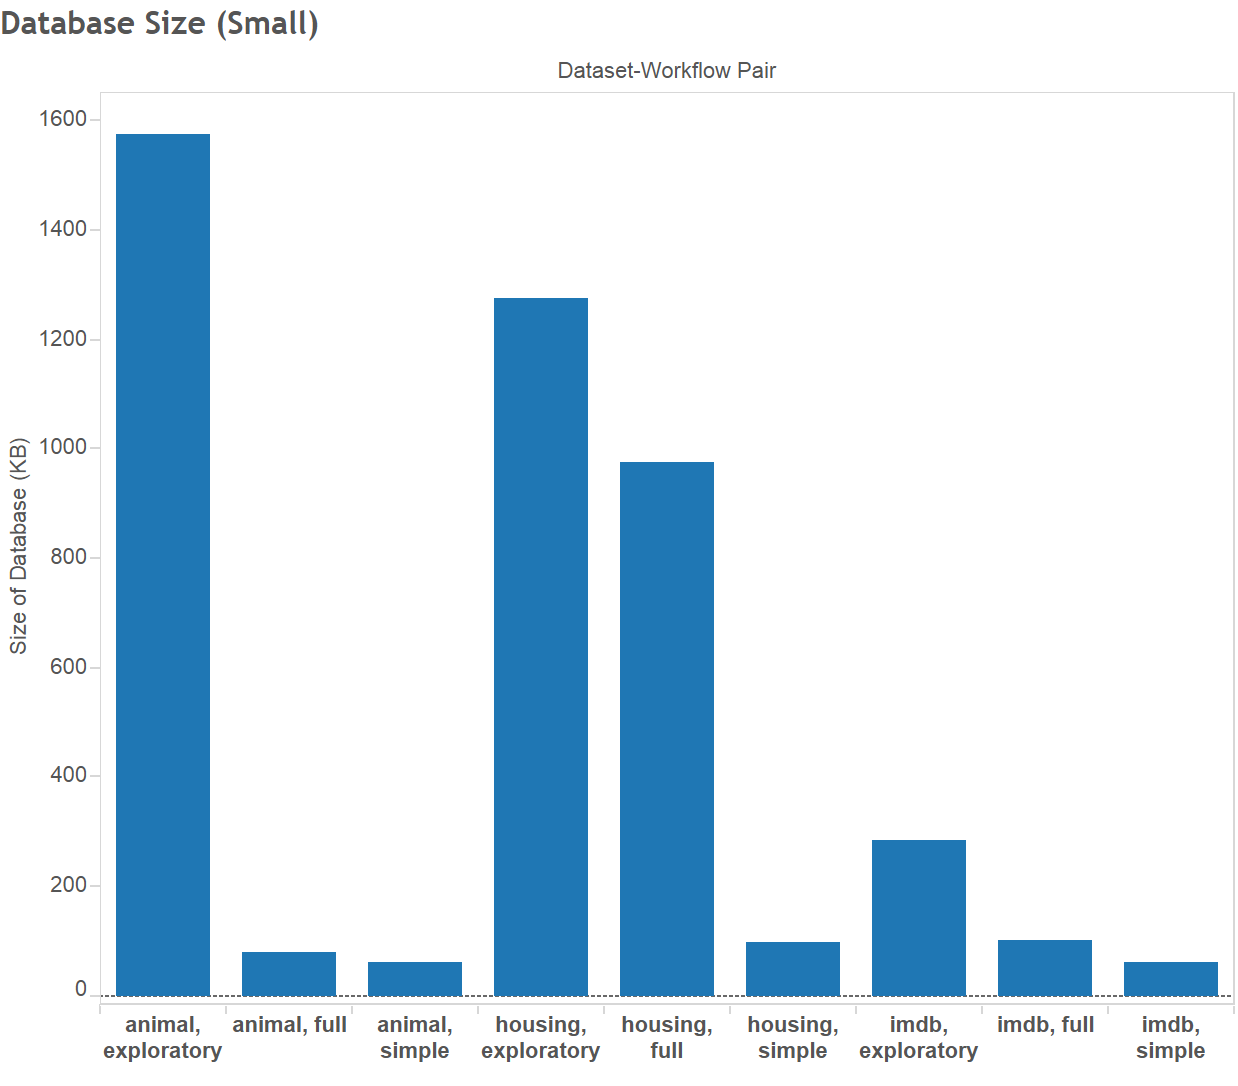
\includegraphics[width=5.0in]{dbsize_small}
  \caption{
    Size of database for each (dataset, workflow) pair when GridSearchCrossValidationEvent intermediates
    are not stored and when the TreeLink and TreeNode tables are only populated for the last model.
  }
  \label{fig:dbsize_small}
\end{figure}


Finally, it is worth looking at the size of the model files produced by each (dataset, workflow) pair. This is shown in
Figure \ref{fig:modelsizes}.

\begin{figure}
  \centering
  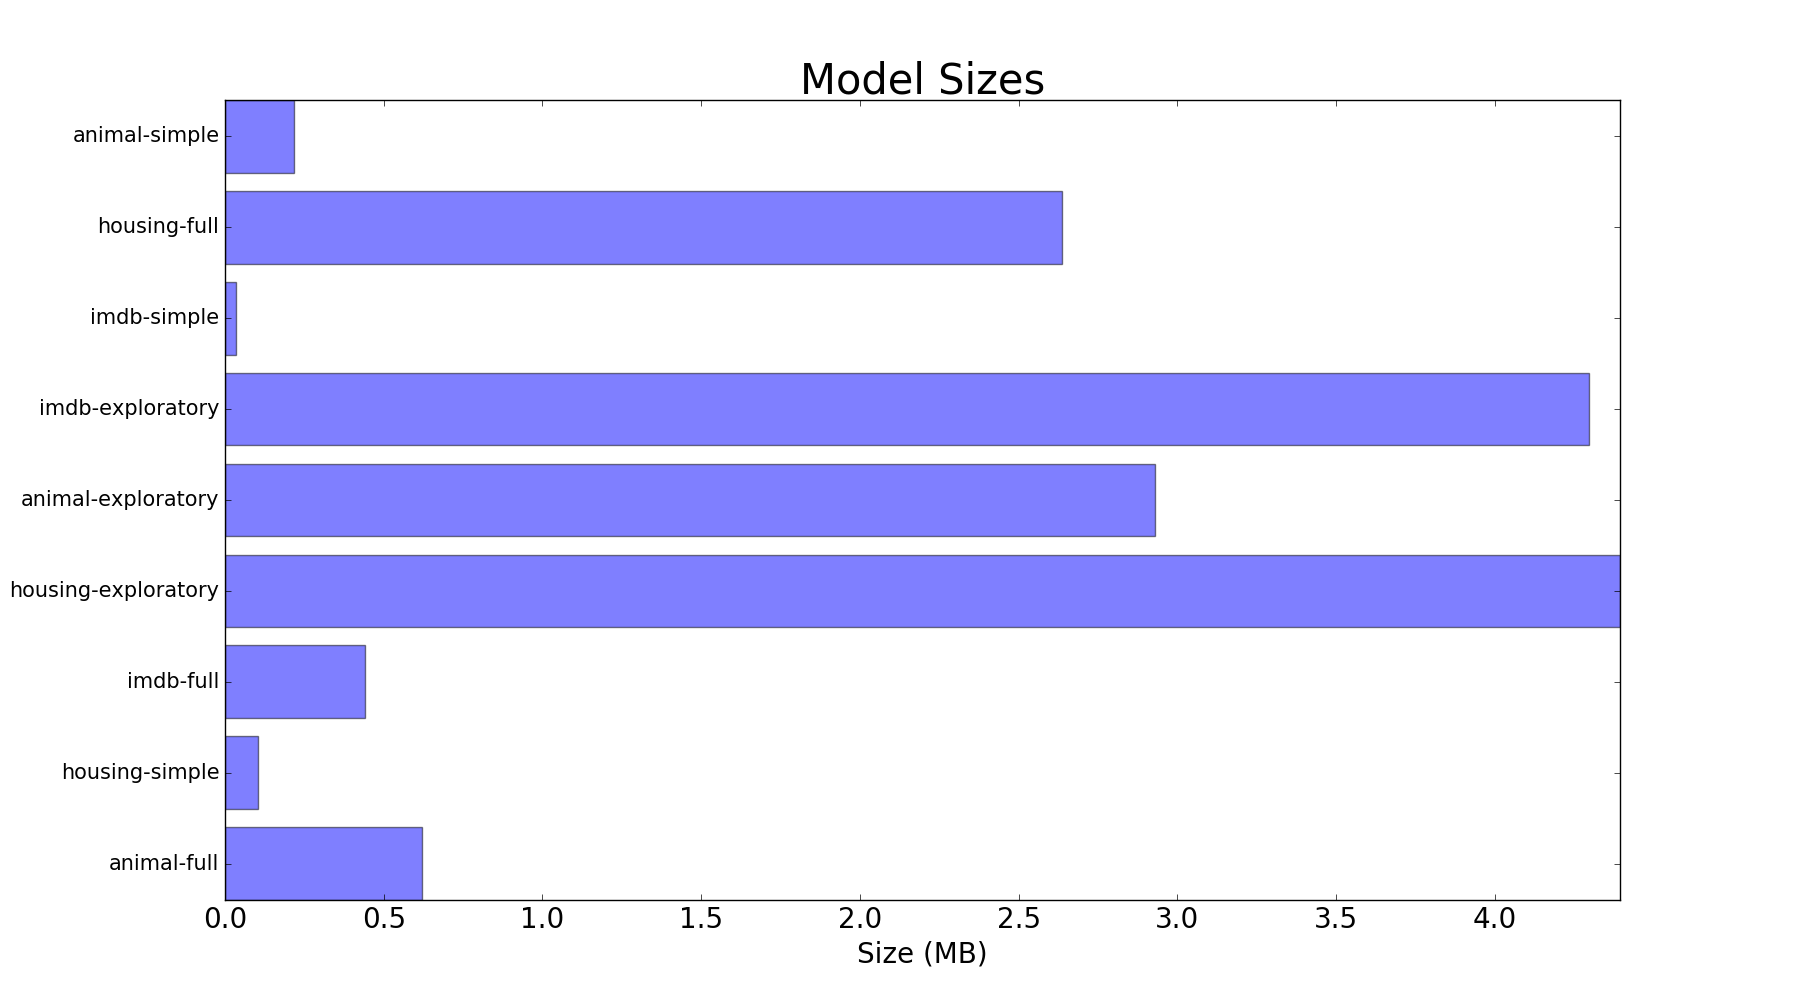
\includegraphics[width=5.0in]{modelsizes}
  \caption{
    Size of model files for each (dataset, workflow) pair.
  }
  \label{fig:modelsizes}
\end{figure}

Again, while these sizes are small (< 5 MB) compared to the size of typical machine learning
datasets, they can still be reduced. Rather than serializing and storing every single model produced in the 
workflow, ModelDB S+C allows the user to indicate which models they would actually like to serialize and store (by
calling saveSync() on the model). When the final models are explicitly serialized and stored, rather than serializing and storing
all the produced Transformers, the model sizes in Figure \ref{fig:modelsizes_small} occur. 

\begin{figure}
  \centering
  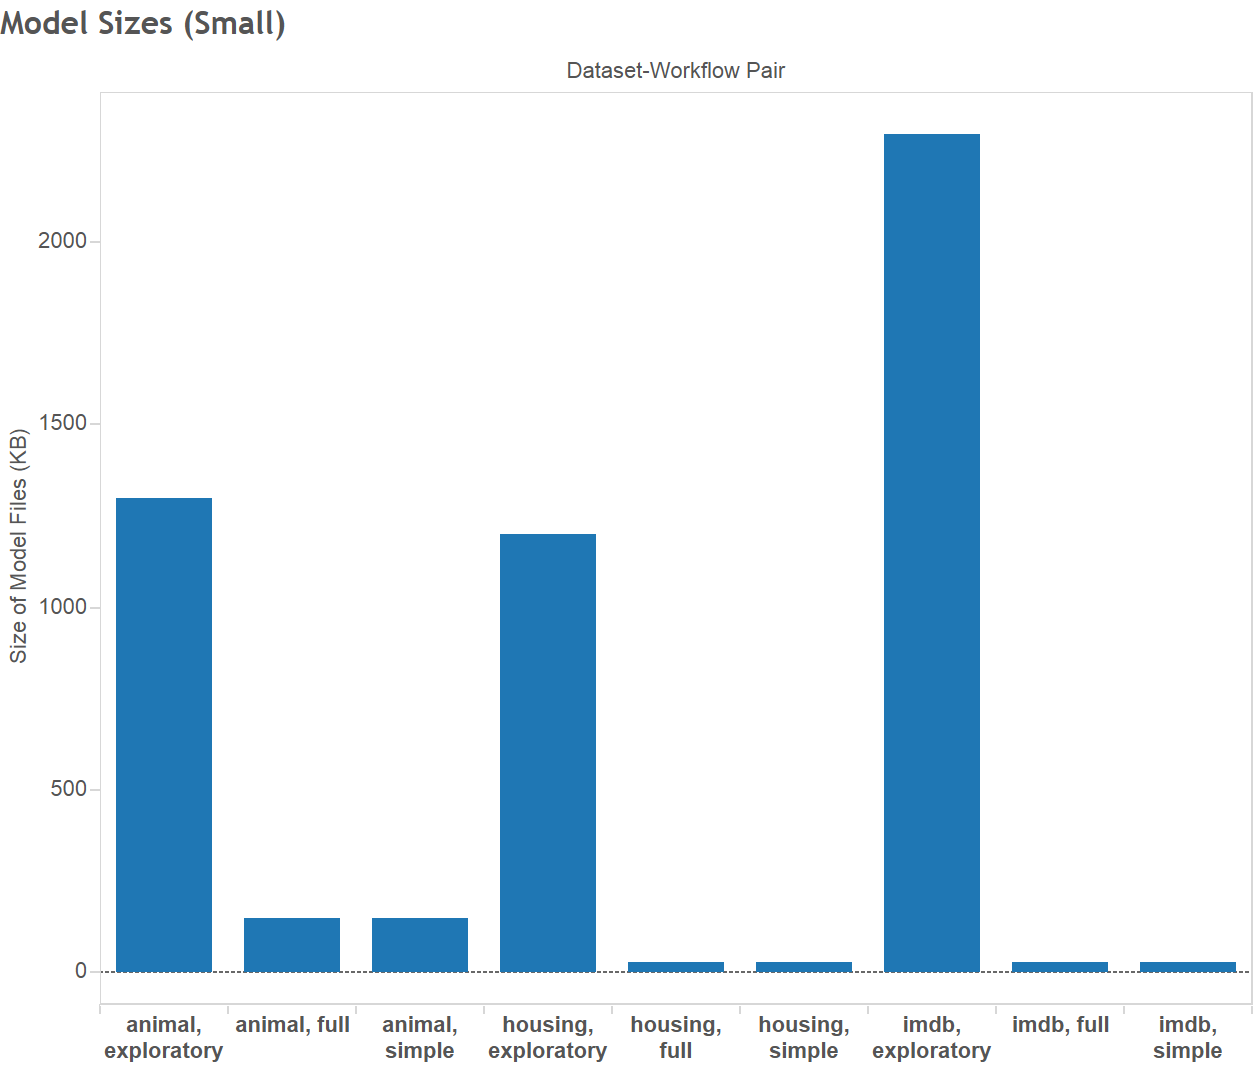
\includegraphics[width=5.0in]{modelsizes_small}
  \caption{
    Size of model files for each (dataset, workflow) pair when only the final models are serialized
    and stored, rather than serializing and storing all produced Transformers.
  }
  \label{fig:modelsizes_small}
\end{figure}

The models in \ref{fig:modelsizes_small} take up much less space.

\section{API Method Time Results}

\section{Model Files Compared to PMML Results}

\section{Evaluating Existing Workflows Results}

\section{Improvements}
